% ^
\documentclass[addpoints,spanish, 12pt,a4paper]{exam}
%\documentclass[answers, spanish, 12pt,a4paper]{exam}
\printanswers
\pointpoints{punto}{puntos}
\hpword{Puntos:}
\vpword{Puntos:}
\htword{Total}
\vtword{Total}
\hsword{Resultado:}
\hqword{Ejercicio:}
\vqword{Ejercicio:}

\usepackage[utf8]{inputenc}
\usepackage[spanish]{babel}
\usepackage{eurosym}
%\usepackage[spanish,es-lcroman, es-tabla, es-noshorthands]{babel}


\usepackage[margin=1in]{geometry}
\usepackage{amsmath,amssymb, cancel}
\usepackage{multicol}
\usepackage{yhmath}

\pointsinrightmargin % Para poner las puntuaciones a la derecha. Se puede cambiar. Si se comenta, sale a la izquierda.
\extrawidth{-2.4cm} %Un poquito más de margen por si ponemos textos largos.
\marginpointname{ \emph{\points}}

\usepackage{graphicx}

\graphicspath{{../img/}} 

\newcommand{\class}{2º Bachillerato CCSS}
\newcommand{\examdate}{\today}
\newcommand{\examnum}{Recuperación Análisis}
\newcommand{\tipo}{A}


\newcommand{\timelimit}{55 minutos}

\renewcommand{\solutiontitle}{\noindent\textbf{Solución:}\enspace}


\pagestyle{head}
\firstpageheader{
\includegraphics[width=0.2\columnwidth]{header_left}}{\textbf{Departamento de Matemáticas\linebreak \class}\linebreak \examnum}{
\includegraphics[width=0.1\columnwidth]{header_right}}
\runningheader{\class}{\examnum}{Página \thepage\ of \numpages}
\runningheadrule


\usepackage{pgf,tikz,pgfplots}
\pgfplotsset{compat=1.15}
\usepackage{mathrsfs}
\usetikzlibrary{arrows}


\begin{document}

\noindent
\begin{tabular*}{\textwidth}{l @{\extracolsep{\fill}} r @{\extracolsep{6pt}} }
\textbf{Nombre:} \makebox[3.5in]{\hrulefill} & \textbf{Fecha:}\makebox[1in]{\hrulefill} \\
 & \\
\textbf{Tiempo: \timelimit} & Tipo: \tipo 
\end{tabular*}
\rule[2ex]{\textwidth}{2pt}
Esta prueba tiene \numquestions\ ejercicios. La puntuación máxima es de \numpoints. 
La nota final de la prueba será la parte proporcional de la puntuación obtenida sobre la puntuación máxima. 

\begin{center}


\addpoints
 %\gradetable[h][questions]
	\pointtable[h][questions]
\end{center}

\noindent
\rule[2ex]{\textwidth}{2pt}

\begin{questions}

\question Calcula los siguientes límites:
\begin{parts}

%https://academico.unizar.es/sites/academico.unizar.es/files/enviodocumento/acceso/armon/matemaplic/acta20191021.pdf

% \part $\lim_{x \to 0}\frac{x+1}{x-1}$
% \begin{solution}$-1$\end{solution}
% \part $\lim_{x \to +\infty}(\sqrt{x}-\sqrt{x-1})$
% \begin{solution}$-1$\end{solution}
% \part $\lim_{x \to 1}\frac{1}{\ln x}$
% \begin{solution}$ \nexists$\end{solution}
% \part $\lim_{x \to 0^+}\ln x$
% \begin{solution}$-\infty$\end{solution}
\part[1] $\displaystyle\lim_{x \to -\infty}e^{x+1}$
\begin{solution}$0$\end{solution}
\part[2] $\displaystyle\lim_{x \to +\infty}\frac{x^2+\sqrt{x+1}}{7x^2-x+4}$
\begin{solution}$\lim_{x \to \infty}\left(\frac{x^{2} + \sqrt{x + 1}}{7 x^{2} - x + 4}\right)=\frac{1}{7}$\end{solution}

\end{parts}


\question Calcular las derivadas de las siguientes funciones: 
\begin{parts}
\part[1] $f(x)=\dfrac{2}{x}+\ln x - \dfrac{\ln x}{x^2}$
\begin{solution}
$\frac{1}{x} - \frac{2}{x^{2}} + \frac{2}{x^{3}} \ln{\left (x \right)}- \frac{1}{x^{3}}$
\end{solution}
\part[1] $g(x)=\dfrac{e^{2x}}{(x+1)^2}$
\begin{solution}
$\frac{2 e^{2 x}}{\left(x + 1\right)^{2}} - \frac{2 e^{2 x}}{\left(x + 1\right)
^{3}}$
\end{solution}
\end{parts}

\question Dada la función, definida para $x \in \mathbb{R} $:
$$f(x)= \begin{cases} 3x+1 &  x < 0 \\ \dfrac{x^2+16}{x+3} & 0\leq x < 5 \\ 
1+2x-\sqrt{4x^2+21} & x \geq 5 \end{cases}$$
\begin{parts}

\part[2] ¿Para qué valores de x es la función f continua?
\begin{solution} 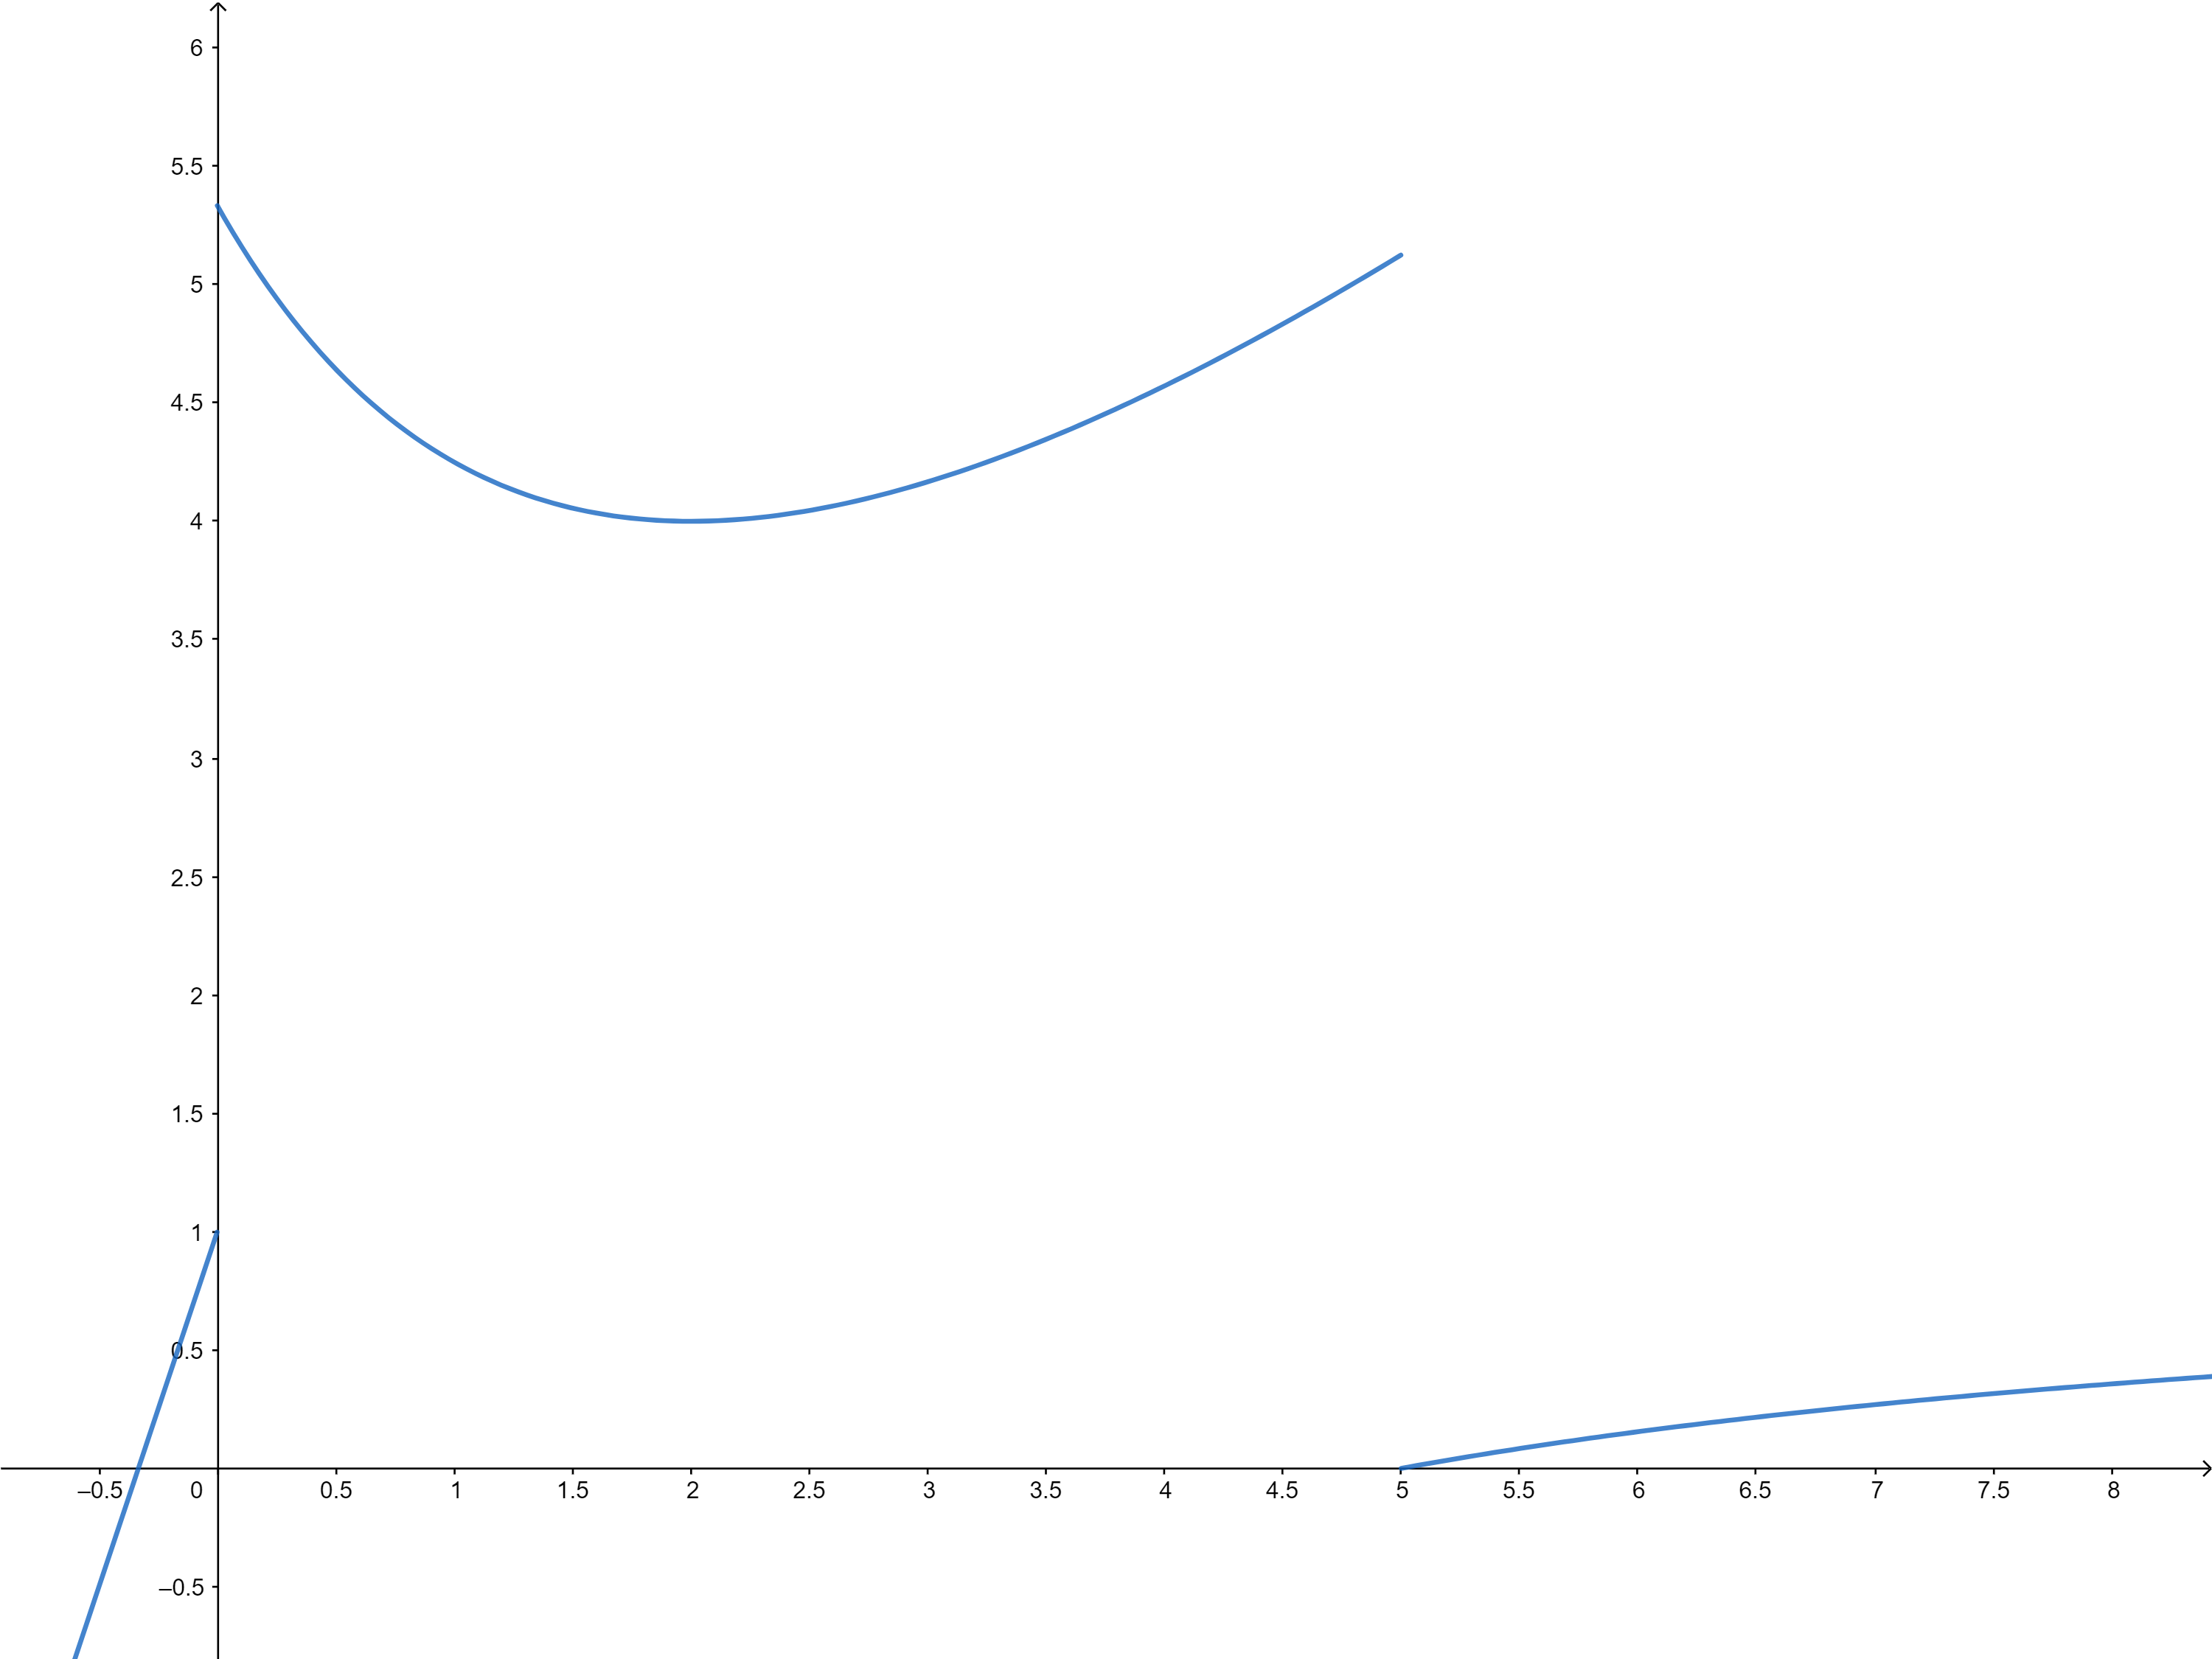
\includegraphics[scale=0.4]{./recan1.png} \\
Para $x \neq 0, 5$ la función es continua y derivable por serlo las funciones parciales \\ 
$\displaystyle\lim_{x \to 0^-} f = 1 \neq \frac{16}{3} = \displaystyle\lim_{x \to 0^+} f \Longrightarrow salto \ finito \ x=0$ \\ 
$\displaystyle\lim_{x \to 5^-} f = \frac{41}{8} \neq 0 = \displaystyle\lim_{x \to 5^+} f \Longrightarrow salto \ finito \ x=5$
\end{solution}
\part[2] Calcular el mínimo valor que toma la función $f$ para $x \in \left[1, 4\right]$
\begin{solution} 
$x \in \left[1, 4\right] \to f'(x)= \frac{2 x}{x + 3} - \frac{x^{2} + 16}{\left(x + 3\right)^{2}}= \dfrac{\left(- x^{2} + 6 x  - 16\right)}{\left(x + 3\right)^{2}}  $\\
$f'(x)=0 \Longleftrightarrow x^{2} + 6 x - 16= 0 \to \cancel{x=-8} \land x = 2 $ \\
$f(1)=\frac{17}{4} \land f(2)=4 \land f(4)=\frac{32}{7} \to min: (2,4)$

\end{solution}
\part[2] Calcular el $\displaystyle\lim_{x \to \infty}f(x)$ 
\begin{solution}$ 1 + 2 x - \sqrt{4 x^{2} + 21} =\frac{(1 + 2 x - \sqrt{4 x^{2} + 21})(1 + 2 x + \sqrt{4 x^{2} + 21})}{1 + 2 x + \sqrt{4 x^{2} + 21}}= \dfrac{4x-20}{1 + 2 x + \sqrt{4 x^{2} + 21}}$\\
$\displaystyle\lim_{x \to \infty}f(x) =\displaystyle\lim_{x \to \infty} \dfrac{4x-20}{1 + 2 x + \sqrt{4 x^{2} + 21}}=\dfrac{4}{2+\sqrt{4}}=1$
\end{solution}
% \part $\displaystyle\lim_{x \to 0^+}\ln x$
% \begin{solution}$-\infty$\end{solution}
% \part $\displaystyle\lim_{x \to +\infty}e^{x+1}$
% \begin{solution}$\infty$\end{solution}
% \part $\displaystyle\lim_{x \to +\infty}\frac{x^2+\sqrt{x+1}}{7x^2-x+4}$
% \begin{solution}$\frac{1}{7}$\end{solution}

\end{parts}



% Reserva 12-13
% \question[1]  Dada la función $f(x) = x^2 + ax + b$, calcular a y b de forma que $f(-1)=3$ y $f$ tenga un mínimo relativo en $x=2$

% \begin{solution}
%     $f(-1)=3 \Longleftrightarrow - a + b + 1 = 3$  \\
%     Mínimo relativo en $x=2 \Longleftrightarrow f'(2)=0 \Longleftrightarrow a + 4 = 0$ \\
%     $\begin{cases}
%     - a + b + 1 = 3   \\
%      a + 4 = 0
%     \end{cases} \to a = -4 \land b=-2$
    
    
% \end{solution}

\question[2]  Dada la función $$f(x) = \dfrac{ax+b}{x^2}$$ Encontrar a y b de forma que $f(1)=2$ y $f$ tenga un máximo relativo en $x=1$

\begin{solution}
    $f(1)=2 \Longleftrightarrow a + b = 2$  \\
    $f'(x)=\dfrac{a}{x^{2}} - \dfrac{2}{x^{3}} \left(a x + b\right)$ \\
    Máximo relativo en $x=1 \Longleftrightarrow f'(1)=0 \Longleftrightarrow - a - 2 b = 0$ \\
    $\begin{cases}
    a + b = 2   \\
    - a - 2 b = 0
    \end{cases} \to a = 4 \land b=-2$
    
    
\end{solution}

\question[2] Calcular $$\int_1^2 \left( 2xe^{3x^2}+\dfrac{6}{x+1}\right) dx$$
\begin{solution}
    $\int_{1}^{2} \left(2 x e^{3 x^{2}} + \frac{6}{x + 1}\right)\, dx=\left[\frac{e^{3 x^{2}}}{3} + 6 \log{\left (x + 1 \right )}\right]_1^2=
    - \frac{e^{3}}{3} - 6 \log{\left (2 \right )} + 6 \log{\left (3 \right )} + \frac{e^{12}}{3}$
\end{solution}

% para comentar ctrl+/ o ctrl+shift+7




\addpoints
\end{questions}

\end{document}

%\grid

